\chapter{Fundamentação Teórica}
\label{cap:fundamentacao-teorica}

\section{Carros Autônomos}
\label{sec:carros autonomos}

Com o avanço da eletrônica e dos \textit{hardwares} tornou-se possível desenvolver veículos que possuem sistemas embarcados e realizam tarefas de forma totalmente independentes, ou seja, autônoma. \cite{rodrigues2017fundamentos}

No brasil, à indústria automobilística representa 18,2\% da economia nacional, segundo dados do G1 \cite{brasilutimorank}. À adoção de padrões de qualidade, o aumento do nível de exigência dos consumidores e à concorrência do mercado são fatores que impactam diretamente na necessidade de inovação dos veículos produzidos, estimulando o investimento em novas tendências tecnológicas. Entre todas essas tendências, é possível afirmar que à condução autônoma é a mais revolucionária da atualidade. Ela mudará toda à concepção de locomoção veicular que temos. \cite{ rodrigues2017fundamentos}

Carro autônomo é um veículo capaz de ler e interpretar o mundo a sua volta através de sensores e câmeras e interagir com ele, locomovendo-se de forma totalmente autônoma e integrando ao sistema de trânsito com segurança e otimização, garantindo a integridade dos seus passageiros e pessoas ao redor.
Os carros autônomos trarão diversos benefícios a sociedade. Uma redução na taxa de acidentes e até no engarrafamento será algo notório quando essa revolução acontecer. Já para os motoristas, um dos maiores atrativos é a possibilidade de realizar outras tarefas enquanto o carro dirige, além de ter uma notória economia de combustível já que ele é controlado por um computador e realiza aceleração e frenagem de forma bem mais preciso que um ser humano. Todos esses fatores se mostraram bastante atraentes para as grandes empresas automobilísticas que entraram com tudo na corrida de desenvolvimento de carros autônomos. \cite{inproceedings,rodrigues2017fundamentos}

Apesar das diversas vantagens dos veículos autônomos, eles ainda terão diversos desafios para entrar no mercado. Dentre eles, as responsabilidades legais sobre os eventos consequentes de suas ações, na qual o veículo não pode ser responsável por possíveis acidentes causados por ele. Para isso, o motorista deve ser responsável por qualquer coisa que venha acontecer e tenha à possibilidade também de monitorar e tomar o controle do veiculo caso seja necessário. \cite{inproceedings}

Outro problema para os veículos autônomos é a legislação de trânsito. Atualmente ela não permite à circulação desses veículos no Brasil. É necessário que haja acréscimo de leis de acordo com as necessidades técnicas e administrativas de cada estado e município.\cite{inproceedings}

Devido à necessidade de sensores, atuadores, dispositivos computacionais e manutenção, os preços dos veículos autônomos são bem mais elevados se comparado aos veículos não autônomos. \cite{inproceedings}

\section{Jaguar}
\label{sec:jaguar}

 O Jaguar é uma Plataforma Robótica Móvel pertencente a Universidade de Fortaleza – Unifor projetada para aplicações que exigem manobrabilidade robusta e manobrabilidade do terreno. Ele possui quatro braços articulados que convertem o Jaguar aos mais variados tipos de configurações de navegação, facilitando a movimentação e até escalada em vários tipos de terrenos \cite{jaguar}. 

Esse robô também possui video e áudio integrados de alta resolução, bateria, GPS, giroscópio e bússola, tudo para ser controlado remotamente por uma rede sem fio 802.11N \cite{jaguar}. 
Essas características tornam o Jaguar uma excelente plataforma para o uso de inteligência artificial. Ele é mostrado na Figura \ref{Jaguar}. A câmera utilizada para a captura das imagens do projeto é apontada pela seta vermelha.

\begin{figure}[H]
	\centering
	\Caption{\label{Jaguar} Jaguar e câmera apontada com seta vermelha}
	\UNIFORfig{}{
		\fbox{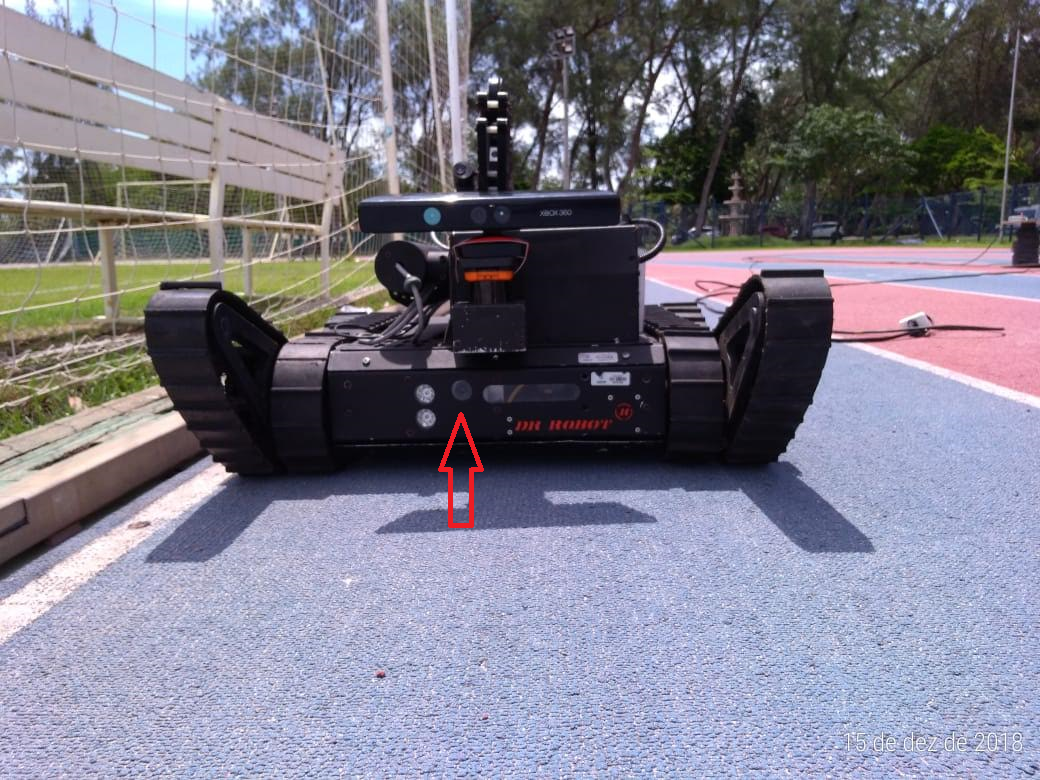
\includegraphics[width=15cm]{figuras/Jaguar.png}}
	}{
		\Fonte{Elaborado pelo autor}
	}	
\end{figure}

\subsection{ROS}

O ROS (\textit{Robotic Operation System}) é uma coleção de \textit{frameworks} de softwares para desenvolvimento de robôs que trabalha com serviços padrões de um sistema operacional, tal como abstração de hardware, controle de dispositivo de baixo nível, passagem de mensagens e gerenciamento de pacotes. Seu funcionamento se baseia em nós, onde cada dispositivo da rede pode ter um ou mais nós e pode enviar ou receber pacotes de dados através da rede do ROS  \cite{ros}.

Um sistema com ROS é constituído por uma série de processos com vários \textit{hosts}, conectados em uma topologia \textit{peer-to-peer}. Eles são conectados via \textit{ethernet} por uma rede \textit{wireless} e precisam de um \textit{host} (que é um nó da rede) mestre ajudar os nós a encontrar outros nós \cite{Ros2}.

O ROS tem suporte nativo a diferentes linguagens:  C ++, Python, Octave, e LISP. Isso é uma forma de facilitar a adaptação dos programadores as ferramentas do ROS. Essas linguagens também possuem bibliotecas para comunicação com o ROS. Além de todas essa facilidades, o ROS é uma ferramenta de código aberto, o que possibilita a adaptação do código e a utilização do mesmo em diversas plataformas \cite{Ros2}.

\section{python}
\label{sec:python}

O python é uma linguagem de alto nível orientada a objetos. Ela se tornou tão popular por causa da sua simplicidade, sintaxe clara e concisa e a sua vasta coleção de módulos prontos para o uso \cite{borges2014python}. 

Além de ser estar nativamente em sistemas operacionais, o \textit{python} é utilizado em vários softwares para automatização de tarefas (como BrOffice.org, PostgreSQL, Blender, GIMP e Inkscape) \cite{borges2014python}. 

Python é uma linguagem que vem conquistando diversos desenvolvedores e empresas, tal como a Google, a NASA, a IBM, a Embratel e o Serpro. Se comparada a outras linguagens computacionais, o python é a que mais oferece bibliotecas para o desenvolvimento de inteligência artificial. Além disso, ela possui uma comunidade de desenvolvedores extremamente ativa, auxiliando o desenvolvimento e aprendizado de novas aplicações nessa linguagem \cite{jonasgranatyr}. 

\section{INTELIGÊNCIA ARTIFICIAL }
\label{sec:INTELIGÊNCIA ARTIFICIAL }

Problemas computacionais sempre foram resolvidos através da programação de
longos códigos, nos quais é especificado cada passo que o computador tem que realizar. Porém, trabalhos que o homem realiza com facilidade pode ser algo bem difícil para ser programado em um computador, como por exemplo o reconhecimento facial, que qualquer acessório ou pequena mudança visual pode dificultar o reconhecimento pelo algoritmo. Essas características, tais como mudança de comportamento, humor e tonalidade da voz são relativamente fáceis de serem percebidas por uma pessoa \cite{lorenafaceli2011inteligencia}. 

%Analise de dados e gráficas são tarefas complexas para serem programadas, principalmente se tiverem que tirar conclusões baseadas nos dados. E, além da complexidade dessas tarefas, é preciso que elas sejam realizadas inúmeras vezes durante um dia. Em alguns casos, o volume de informação é tão grande que se torna impossível de ser analisado por seres humanos \cite{lorenafaceli2011inteligencia}. 
 
Inteligência artificial então é o ramo da computação que procura, por meios computacionais, desenvolver capacidades semelhantes à dos seres humanos para uma máquina, tais como: raciocinar, planejar, resolver problemas, armazenar conhecimento, aprender, perceber e adaptar-se ao meio. \cite{Fernando}.

\section{Aprendizado de Máquina}
\label{sec:aprendizado de máquina}

Estamos em um tempo onde \textit{terabytes} de informações (dados) são criados diariamente. Esses dados podem ser de dois tipos: estruturados (completos sem faltar informação, deixando-o fácil de ser localizado) e não-estruturado (faltando alguma informação nos dados dificultando a sua localização). Se bem trabalhados e analisados, esses dados podem fornecer um grande conhecimento. Cabe então ao algorítimo de \acrlong{ML} (ML) trabalhar com esses dados para fazer previsões \cite{pythonmachinelearning}. 

Grandes empresas, como Google, Apple, Amazon, IBM, Microsoft, Facebook e Twitter já usam essa incrível tecnologia. Elas utilizam o Aprendizado de Máquina (Aprendizado de máquina em inglês) para conhecer melhor os seus usuários e fornecer um melhor serviço \cite{pythonmachinelearning}. Um grande exemplo de uso do ML é na análise de sentimentos, onde é possível saber a reação (positiva ou negativa) dos usuários de uma determinada rede social sobre um determinado assunto \cite{sentimentos}.

O algoritmo de Aprendizado de Máquina aprende padrões a partir dos dados entrada juntamente com os seus dados de saída. e pode treinar a máquina para realizar tarefas de forma autônoma. \cite{diferencamachinelearning}.

Em relação ao tipo de aprendizagem, o algoritmo de Aprendizado de Máquina pode ser classificado em três tipos: Aprendizagem Supervisionada (\ref{aprendizadagem supervisionada}), Aprendizagem não supervisionada (\ref{Aprendizagem não supervisionada}) e Aprendizagem por Reforço (\ref{Aprendizagem por Reforço}).

\subsection{Aprendizagem Supervisionada}
\label{aprendizadagem supervisionada}
Nesse tipo de aprendizagem é fornecido para o computador dados rotulados, ou seja, dados de entrada com a sua saída já conhecida. Com isso, é possível prever dados futuros \cite{pythonmachinelearning}. 
A Aprendizagem Supervisionada pode ser dividida em dois modelos regressão e classificação. No caso da regressão, os dados de entrada são utilizados para criar uma função que gere um valor contínuo. No caso da classificação os dados de entrada são utilizados para mapear os dados de saída em classificações distintas \cite{pythonmachinelearning}. 

\subsection{Aprendizagem não supervisionada}
\label{Aprendizagem não supervisionada}
No caso da Aprendizagem não supervisionada o algoritmo irá trabalhar com dados de entrada nos quais não há praticamente nenhum dado de saída ligado a eles. Ou seja, a máquina terá que gerar uma classificação com a entrada, determinado um padrão entre eles \cite{pythonmachinelearning}. Problemas como esse são normalmente mais complexos principalmente por que não há uma resposta para os dados de teste, tornando assim difícil de avaliar o modelo resultante desse aprendizado.

\subsection{Aprendizagem por Reforço}
\label{Aprendizagem por Reforço}
Através de tentativas e erros, o algoritmo de Aprendizado de Máquina vai procurar uma melhor forma de atuar no ambiente de trabalho para encontrar o sinal de recompensa. Por meio da interação, a máquina procura uma série de ações que levam, da melhor maneira possível, a uma determinada recompensa e reduza o erro. Um exemplo dessa aprendizagem é o jogo de xadrez, onde o algoritmo decide, entre uma série de movimentos e o estado do tabuleiro, quais deles vão levar a máquina para vitória e distancia-la da derrota \cite{pythonmachinelearning}.

\section{Aprendizagem Profunda}
\label{deep learning}

Aprendizagem Profunda (DL) é uma forma de aprendizagem de máquina que permite que o computador aprenda através de experiências passadas e compreenda o mundo por uma ideia de hierarquia e conceitos, onde cada nível dessa hierarquia é utilizado para definir outro nível hierárquico. Nesse tipo de aprendizagem não é necessário um operador vistoriando e especificando os conhecimentos necessários para o computador já que ele aprende com experiências passadas. A hierarquia de conceitos permite que o computador aprenda os conceitos complicados de forma mais simples \cite{goodfellow2016deep}. Então, \acrlong{DL} (DL) pode ser dito como uma subcategoria do Aprendizado de Máquina que, por meio de algoritmos mais complexos, imita a rede neural do cérebro humano \cite{diferencamachinelearning}.

Esse tipo de apredizagem utiliza redes neurais artificiais como base do seu algoritmo, porém com muito mais camadas (\textit{Layers}). Foi através dessa subcategoria que tornou-se possível avanços na visão computacional, reconhecimento de fala, processamento de linguagem natural e reconhecimento de áudio.

\section{Redes Neurais Artificiais}
\label{redes neurais}

\acrlong{ANN} (ANN) é um modelo computacional inspirado pela própria organização biológica do processamento de informação do cérebro humano. São algoritmos que aprendem a modelar uma relação entre a entrada e saída dos dados. esses algoritmos são comumente utilizados para reconhecimento de padrões no campo da medicina, ciências puras, negócios, mineração de dados \cite{redeneuralnvidia}.

À unidade básica da ANN é chamada de nó, unidade ou neurônio, seu nome mais popular. Por sua vez, ele recebe à entrada de outros nós ou uma fonte externa para gerar uma saída. Dentro do nó há uma função(f) que determina o valor de sua saída e um peso(w) que é calculado de acordo com sua importância em relação aos outros nós. Uma ideia ilustrativa é mostrada na Figura \ref{neuronio} \cite{conv2,redeneuralnvidia}.

\begin{figure}[H]
	\centering
	\Caption{\label{neuronio}Neurônio}
	\UNIFORfig{}{
		\fbox{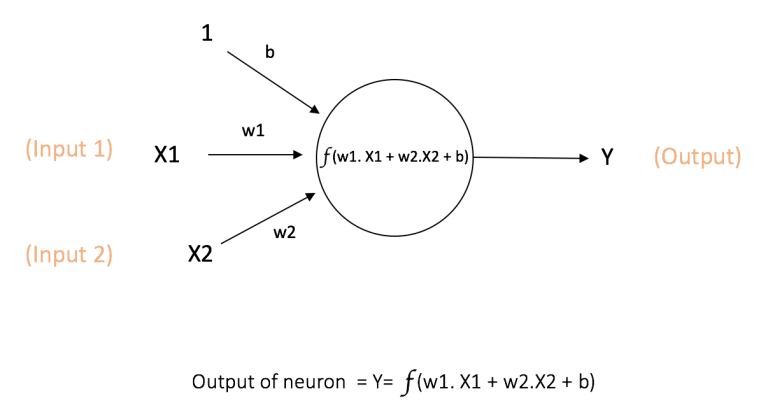
\includegraphics[width=15cm]{figuras/neuralnetwork.png}}
	}{
		\Fonte{\cite{conv2}}
	}	
\end{figure}

Nessa rede o neurônio recebe X1 e X2 nas suas entradas e à atribuição dos pesos w1 e w2, respectivamente. Na entrada 1 há uma Bias chamado b. Ela soma um determinado valor calculado pela propia ANN na função de ativação. Sua saída Y é calculada pela função f, conhecida como função de ativação, que tem por finalidade introduzir a saída de um neurônio a não-linearidade, já que os dados do mundo real são não-lineares. Cada neurônio possui uma função de ativação com valores únicos \cite{conv2}.

Na Rede neural, cada neurônio de uma camada é ligado à um neurônio da camada seguinte. No processo de aprendizagem, o \textit{dataset} de entrada vai passando por todas as camadas mudando as variáveis (os pesos e padrões) das funções de entrada de forma que minimize ao máximo a diferença entre os valores desejados e as previsões da rede neural \cite{redeneuralnvidia}.

O primeiro tipo de rede neural desenvolvido foi a \textit{Feedforward}, que é também o mais simples. Essa ANN possui três tipos de camadas: camada de entrada, camada escondida e camada de saída. Ela funciona basicamente com um caminho único para o \textit{dataset} onde ele entra pela camada de entrada e vai percorrendo todas as camadas até a camada de saída, não existindo assim nenhum ciclo de retorno ou \textit{loop} na rede \cite{conv2, redeneuralnvidia}.

Redes Neurais Artificiais \textit{Feedforward} são divididas em dois tipos: \textit{Single Layer Perceptron}, onde ela possui apenas a camada de entrada e saída, e \textit{Multi Layer Perceptron}, que tem todas as três camadas (camada de entrada, camada de saída e camada escondida), podendo ter uma ou mais camada escondida. Esse é o modelo de ANN utilizado para Redes Neurais Convolucionais, explicada no tópico \ref{redes neurais convolucionais} \cite{redeneuralnvidia}.

\section{Redes Neurais Convolucionais}
\label{redes neurais convolucionais}

\acrlong{CNN} (também conhecida como ConvNet ou CNN) é um tipo de rede neural artificial que pode receber uma imagem de entrada e atribuir diferentes graus de importância para vários aspectos ou objetos da imagem, diferenciando um do outro. O pré-processamento de uma rede neural desse tipo é relativamente menor, se comparado aos outros algoritmos de classificação, já que à CNN tem à capacidade de “aprender” o filtro de classificação, enquanto os outros algoritmos necessitam que o filtro seja todo escrito pelo programador\cite{redesneuraisconv,deeplearningbook}.

A primeira proposta de um projeto de rede neural convolucional foi feita em 1988, por Yann LeCun. Seu nome era \textit{LeNet} e era utilizada para o reconhecimento de características numéricas. Ela foi de grande utilidade para impulsionar o campo de pesquisa de Aprendizagem Profunda \cite{redesneuraisconv}.

Os algoritmos de CNN podem dar capacidade ao computador de ver o mundo como um ser humano, conseguindo distinguir diferentes objetos e aspectos da imagem em análise. À Figura  \ref{keras_exemple} mostra um exemplo disso, no qual  o algoritmo consegue, com alta taxa de precisão, distinguir os diferentes conteúdos da imagem \cite{conv1,conv2}.

\begin{figure}[H]
	\centering
	\Caption{\label{keras_exemple} Exemplo de reconhecimento de Objetos de uma CNN}
	\UNIFORfig{}{
		\fbox{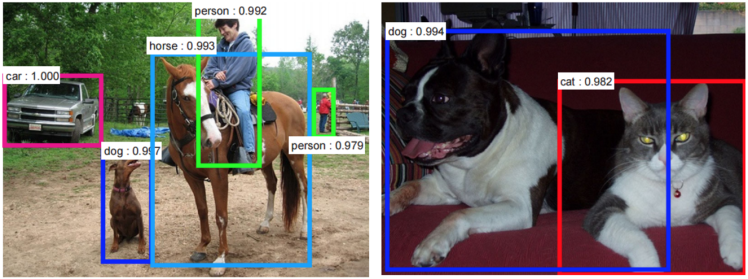
\includegraphics[width=15cm]{fig/keras_exemple.png}}
	}{
		\Fonte{\cite{conv2}}
	}	
\end{figure}

Existem diversas bibliotecas que realizam à implementação de uma Rede Neural Convolucional: \textit{Caffe, MatConvNet, Theano, Torch}. Para esse projeto foi utilizado a bibliteoca \textit{Keras} que é uma API de alto nível desenvolvido em python e baseado no \textit{Tensorflow}, biblioteca de aprendizado de máquina  e de código aberto desenvolvida pelo \textit{Google Brain}, em 2015 \cite{redesneuraisconv,keras,tensorflow}.

A arquitetura de uma CNN é semelhante ao padrão de conectividade dos neurônios dos seres humanos, sendo inspirada na organização do Cortex. \cite{conv1}

 As CNNs possuem diversas camadas, mas há sempre três principais: convolucionais, \textit{pooling} e totalmente conectada. A camada convolucional possui diversos neurônios que tratam de aplicar um filtro em uma determinada parte da imagem. A camada de \textit{pooling} trata de reduzir o tamanho da imagem e fazer a ativação dos pixels mais significativos e a camada totalmente conectada faz a classificação. A Figura \ref{exemplo_cnn} mostra uma ilustração de uma CNN.

\begin{figure}[H]
	\centering
	\Caption{\label{exemplo_cnn} Ilustração de uma CNN}
	\UNIFORfig{}{
		\fbox{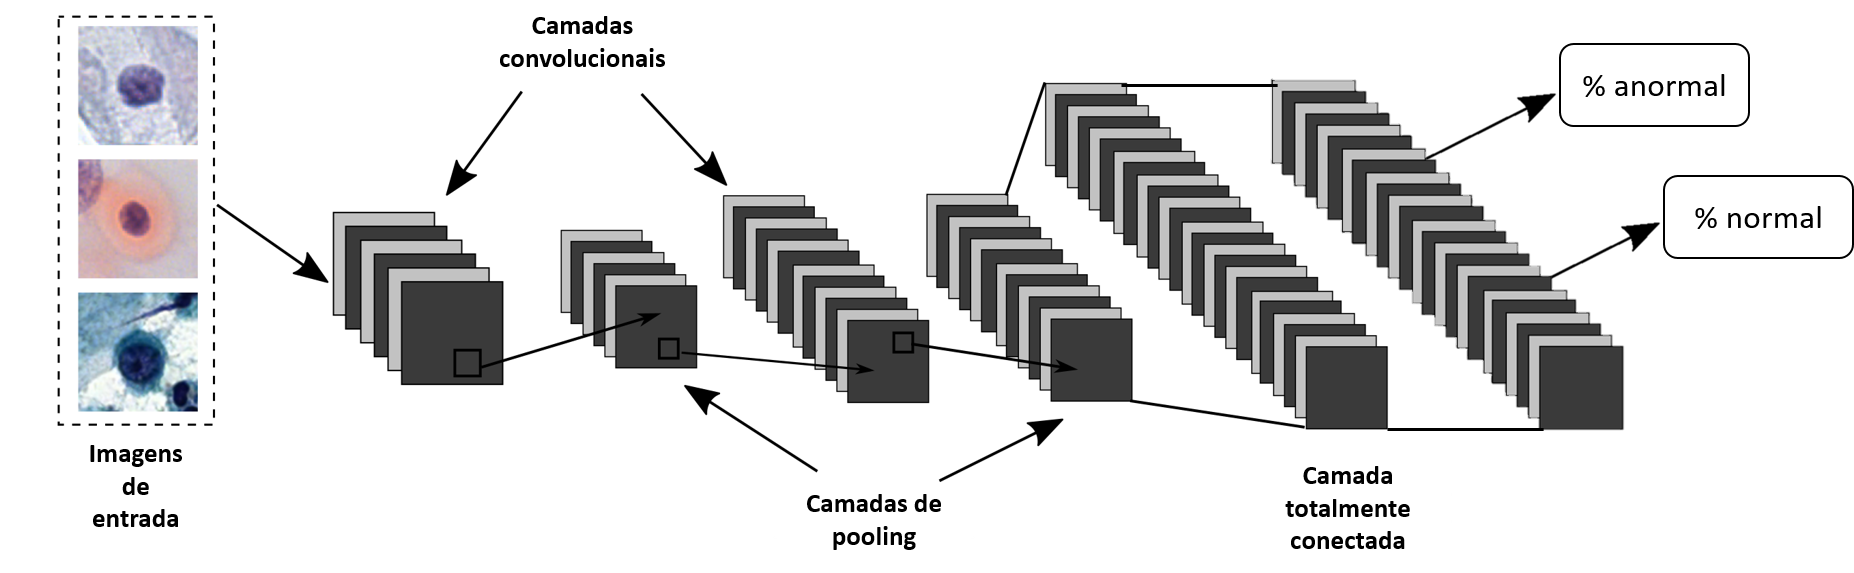
\includegraphics[width=15cm]{fig/exemplo_CNN.png}}
	}{
		\Fonte{\cite{redesneuraisconv}}
	}	
\end{figure}

O volume de entrada que o algoritmo de CNN irá trabalhar é uma imagem. Para entender o funcionamento do algoritmo é preciso primeiramente entender o que é uma imagem na visão computacional\cite{conv2}. 

Basicamente é possível dizer que uma imagem é uma matriz de valores de pixel. Cada valor dessa matriz possui três canais: vermelho, verde e azul, no qual cada um possui um número de 0 a 255 para assim poder formar as cores de cada pixel da imagem. Para imagens em preto e branco existem apenas um canal que também vai de 0 á 255, porém apenas na escala de cinza. 
Com essa visão básica de como é formado uma imagem, é possível compreender como cada uma das camadas da rede neural trabalham.

\subsection{Camada Convolucional}

É a primeira camada da CNN. Sua função reduz o tamanho da imagem sem perder suas principais características que são fundamentais para a predição. Para isso, é possível utilizar quantas camadas for necessário \cite{freecodecamp}. É uma camada que consiste em um conjunto de filtros (também conhecidos como \textit{kernels}), que são configurados pela própia CNN enquanto ela vai recebendo dados de entrada, nos quais eles recebem como entrada um arranjo tridimensional, também chamado de volume. Nessa camada nem sempre os neurônios são conectados a todos os neurônios da camada seguinte, como na Rede Neural. Eles se conectam à apenas uma pequena região do mesmo. Conforme a imagem passa por cada camada convolucional ela vai reduzindo assim como o seu filtro \cite{freecodecamp, conv2}.
 
 Uma imagem retirada de um video \textit{Full HD} tem uma resolução de 1920 x 1080 \textit{pixels}, ou seja, 1920 \textit{pixels} na largura e 1080 \textit{pixels} na altura, no qual cada um desses \textit{pixels} há três canais de cores com 256 tonalidades para cada um \cite{resolucao}. Por questões de didáticas, será utilizado um exemplo mais simples de resolução 5 x 5 e apenas um canal de cor com 2 tonalidades.
 \begin{figure}[H]
	\centering
	\Caption{\label{filtro1} Volume de entrada e o Filtro}
	\UNIFORfig{}{
		\fbox{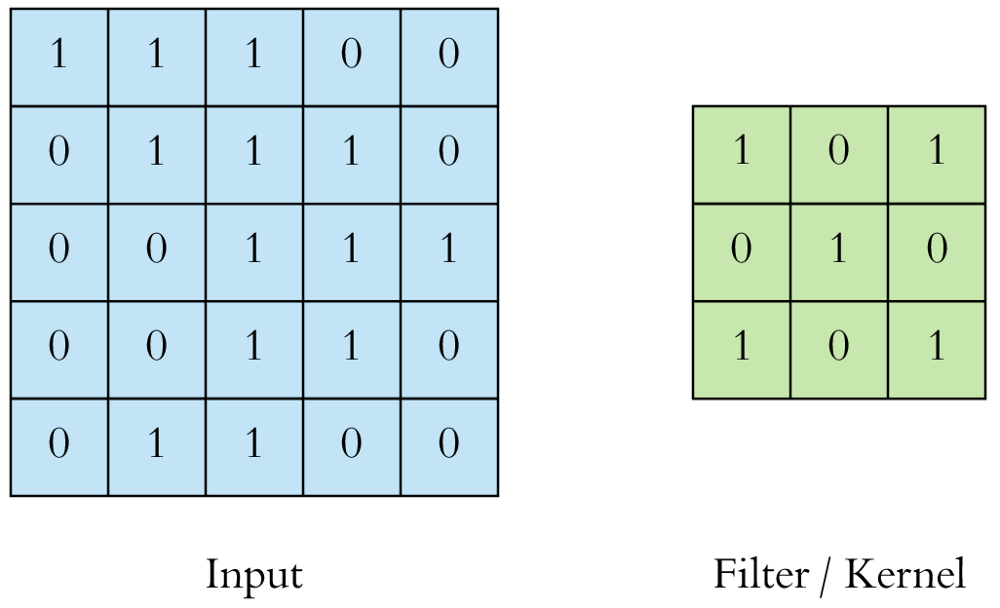
\includegraphics[width=12cm]{fig/filtro3.png}}
	}{
		\Fonte{\cite{freecodecamp}}
	}	
\end{figure}

Na Figura \ref{filtro1} temos a Imagem de entrada representada pelo \textit{Input}, onde cada \textit{pixel} é representado por um quadrado da figura e o seu filtro representado por \textit{Filter/Kernel}. O filtro irá passar sobre essa imagem, da esquerda para direta, fazendo o cálculo da matriz da imagem com a matriz do filtro, resultando num mapa de recursos (ou \textit{feature map}), como mostrado na Figura \ref{filtro2} \cite{conv2}.

 \begin{figure}[H]
	\centering
	\Caption{\label{filtro2} Mapa de recursos 1}
	\UNIFORfig{}{
		\fbox{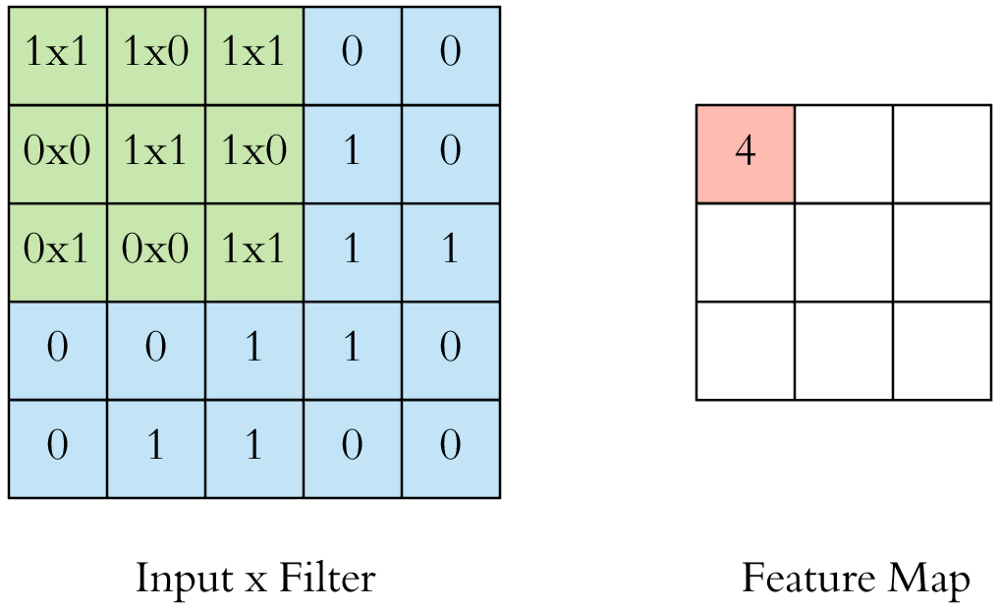
\includegraphics[width=12cm]{fig/filtro2.png}}
	}{
		\Fonte{\cite{freecodecamp}}
	}	
\end{figure}

O filtro percorre, da esquerda para direta e de pixel por pixel, fazendo a multiplicação dos \textit{pixels} da imagem pelos \textit{pixels} do filtro e somando o resultado para criar o mapa de recursos que tem uma linha de pixel a menos em cada um dos seus lados. Esse movimento é repetido linha por linha da imagem de entrada. O resultado Final é mostrado na Figura \ref{filtro3} \cite{conv2, freecodecamp}.

 \begin{figure}[H]
	\centering
	\Caption{\label{filtro3} Mapa de recursos 2}
	\UNIFORfig{}{
		\fbox{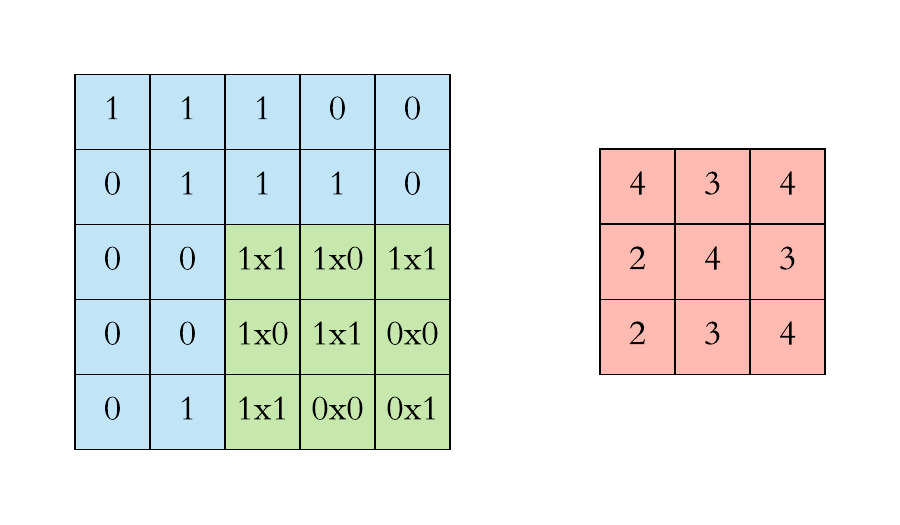
\includegraphics[width=12cm]{fig/filtro4.jpg}}
	}{
		\Fonte{\cite{freecodecamp}}
	}	
\end{figure}

Os filtros podem possuir diferentes valores, gerando assim diferentes efeitos convolucionais. Com isso é possível realizar operações como detecção de borda, nitidez e borrão com apenas uma mudança de valores numéricos da sua matriz. A Figura \ref{filtro4} mostra exemplos de algumas operações. Elas são descritas na primeira coluna (identidade, detecção de bordas, aguçamento e borrão, em ordem). Na coluna do meio tem a matriz do filtro e o resultado convolucional na última coluna. Os  valores dos filtros são aprendidos pela CNN, mesmo ainda sendo preciso especificar alguns parâmetros pelo programador como número, tamanho, arquitetura do filtro \cite{conv2, aprendizadoDeMaquinaDivertido}.

\begin{figure}[H]
	\centering
	\Caption{\label{filtro4} Diferentes tipos de Filtros}
	\UNIFORfig{}{
		\fbox{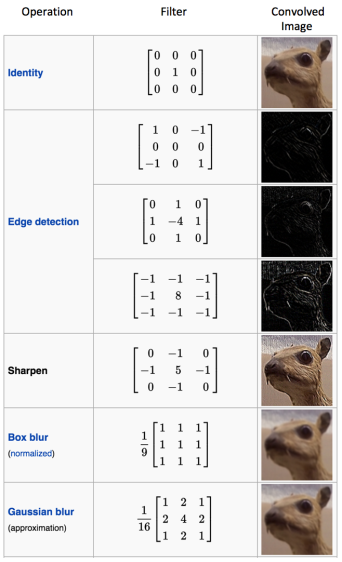
\includegraphics[width=10cm]{fig/tiposdefiltros.png}}
	}{
		\Fonte{\cite{conv2}}
	}	
\end{figure}

O resultado final da convolução, o \textit{feature map} é controlado por três parâmetros:
\begin{description}
    \item[Profundidade:] é o número de filtros usado para a convolução.
    \item[\textit{Stride:}] é o número de \textit{pixel} que o filtro vai percorrer por vez. Por exemplo: se o \textit{Stride} for igual a 1, o filtro vai percorrer apenas 1 pixel por vez.
    \item[\textit{Zero-padding:}] em alguns casos é preciso preencher a borda da matriz de entrada (a imagem) com zeros para poder controlar o tamanho do mapa de características. 
\end{description}

Ao final de cada operação de convolução também é comum utilizar uma função de não-linearidade, a ReLU. Sua função é substituir todos os \textit{pixels} negativos por zero do mapa de recursos. Então, a \acrlong{ReLU} (ReLU) introduz a não-linearidade no resultado final já que a maioria dos dados de entrada reais são não-lineares \cite{conv2}.
A Figura \ref{filtro6} mostra um exemplo da aplicação dessa função, onde a imagem da direita é o resultado depois da aplicação da mesma.

\begin{figure}[H]
	\centering
	\Caption{\label{filtro6} Aplicação da função ReLU}
	\UNIFORfig{}{
		\fbox{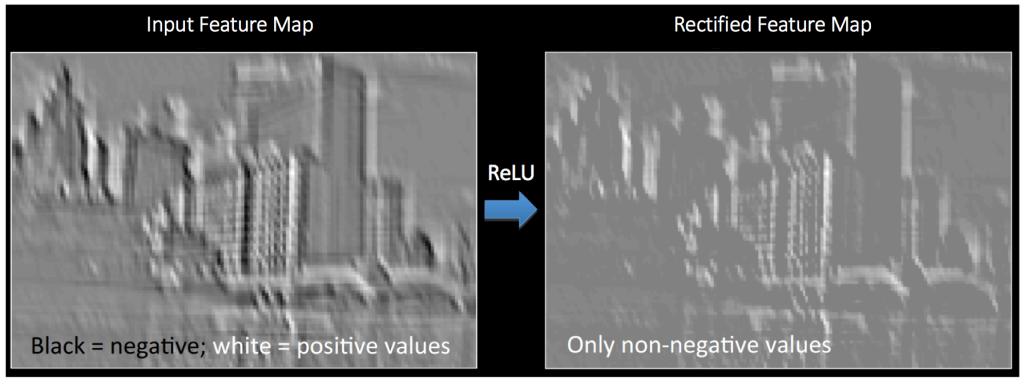
\includegraphics[width=16cm]{fig/relu.png}}
	}{
		\Fonte{\cite{conv2}}
	}	
\end{figure}

Para esse projeto foi utilizado a função de ativação ELU (\acrlong{ELU}, ou inglês, \acrlong{ELU2}). Ela converge mais rapidamente para o zero e possui resultados mais precisos.

Em relação ao ReLU, ela possui uma constante extra positiva, chamada de alfa. Ela também difere do ReLU pela sua suavização, que é mais lente e bem menos acentuada. É possível ver isso no gráfico da Figura \ref{elurelu} \cite{elu}.

\begin{figure}[H]
	\centering
	\Caption{\label{elurelu} Função Elu x ReLU}
	\UNIFORfig{}{
		\fbox{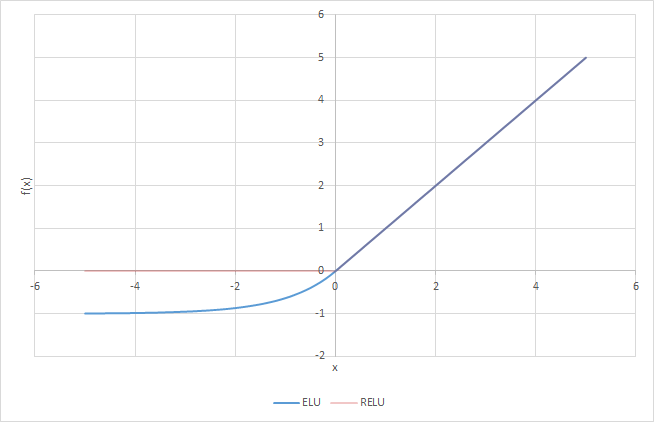
\includegraphics[width=15cm]{fig/elurelu.png}}
	}{
		\Fonte{\cite{elu}}
	}	
\end{figure}

\subsection{Camada de \textit{Pooling}}

A função da camada de \textit{pooling} (também chamada de subamostragem ou \textit{downsampling}) é reduzir a dimensão do mapa de recursos mantendo as informações mais importantes. Podemos ter a soma, a média ou \textit{Max Pooling}, que é a mais popular e também utilizada nesse trabalho. Essa última funciona definindo uma janela de \textit{pixels} (por exemplo, uma janela 2x2 onde ela "visualiza" apenas 4 \textit{pixels} do mapa de amostragem) e seleciona o maior deles para montar outro mapa de recursos, como é mostrado na Figura \ref{maxpool}. Essa função se aplica por toda a imagem \cite{freecodecamp}.

\begin{figure}[H]
	\centering
	\Caption{\label{maxpool} Aplicação do \textit{Pooling}}
	\UNIFORfig{}{
		\fbox{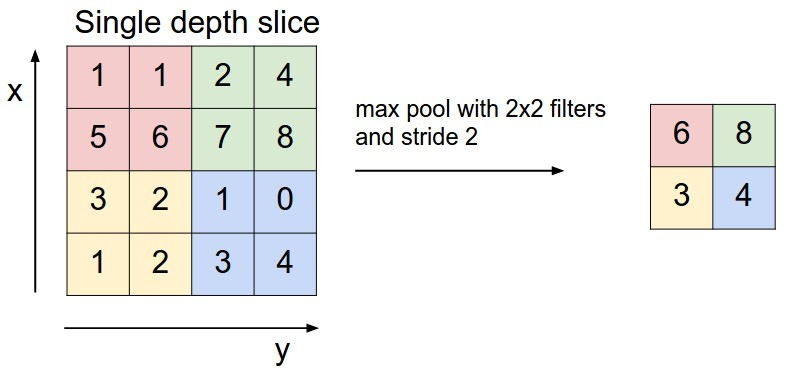
\includegraphics[width=15cm]{fig/maxpool.jpg}}
	}{
		\Fonte{\cite{CS231n}}
	}	
\end{figure}

O resultado da aplicação dessa camada é mostrado na Figura \ref{pool} (lembrando que já foi aplicado a convolução e ativador ReLU na imagem).

\begin{figure}[H]
	\centering
	\Caption{\label{pool} Exemplo de \textit{Pooling}}
	\UNIFORfig{}{
		\fbox{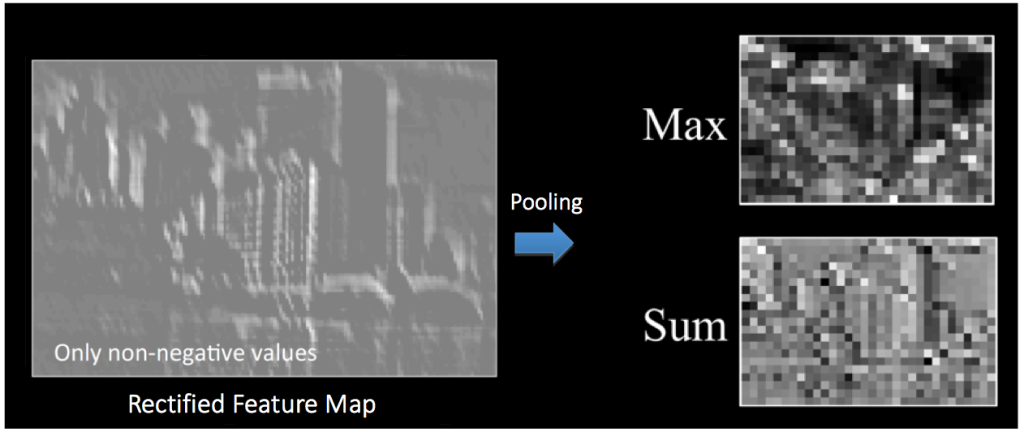
\includegraphics[width=15cm]{fig/pool.png}}
	}{
		\Fonte{\cite{conv2}}
	}	
\end{figure}

\subsection{Camada Totalmente Conectada}

Camada totalmente conectada é uma camada onde todos os neurônios da camada anterior estão totalmente conectados a todos os neurônios da camada posterior. Seu objetivo é classificar as imagens de entrada nos vários grupos determinados pelo \textit{dataset}. Essa é etapa final da predição, onde ela irá retornar um valor para o usuário entre 0 (0\% de probabilidade) e 1 (100\% de probabilidade) referente a cada um dos \textit{datasets}. A Figura \ref{exemploCNN} mostra, na sua extremidade direita, o percentual de probabilidade de ser cada um dos \textit{datasets} inseridos. Pode-se observar que o \textit{boat} (barco) tem a maior probabilidade, sendo 0,94.\cite{conv2, aprendizadoDeMaquinaDivertido}. 
Lembrando que essas são as camadas básicas de uma CNN, mas não necessariamente elas precisam sempre seguir essa Ordem. Na Figura \ref{exemploCNN}, por exemplo, há duas camadas Convolucionais com ReLU e \textit{Pooling} para no final haver duas camadas totalmente conectadas \cite{conv2}.

\begin{figure}[H]
	\centering
	\Caption{\label{exemploCNN} Exemplo de Rede Neural Convolucional}
	\UNIFORfig{}{
		\fbox{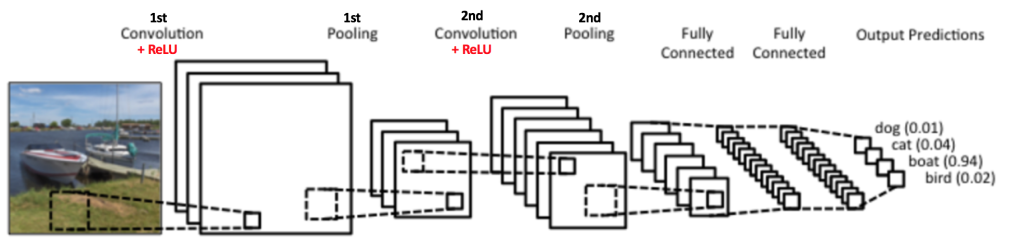
\includegraphics[width=16cm]{fig/exemploCNN.png}}
	}{
		\Fonte{\cite{conv2}}
	}	
\end{figure}
